
\begin{table*}[htbp]
\centering
\scriptsize
\setlength{\tabcolsep}{1.5pt}
% \resizebox{1\textwidth}{!}{
\begin{tabular}{l|c|cccccc|ccc|c|c|c}
\toprule
\multirow{2}{*}{\textbf{Methods}}  & 
\multirow{2}{*}{\renewcommand{\arraystretch}{0.8}\begin{tabular}[x]{@{}c@{}}\textbf{Fine-}\\ \textbf{Tuning}\\\textbf{Free}\end{tabular}} & 
\multicolumn{6}{c|}{\textbf{\textit{Unseen Center}}} &  \multicolumn{3}{c|}{\textbf{\textit{Unseen Organ}}} &  \multicolumn{1}{c|}{\textbf{\textit{Unseen Species}}} & \multicolumn{1}{c|}{\textbf{\textit{Unseen Modality}}} & \multirow{2}{*}{\textbf{Average}}  \\
 &  & 
\renewcommand{\arraystretch}{0.8}\begin{tabular}[x]{@{}c@{}}Cerebral\\Cortex\end{tabular}& 
Hippocampus & 
Thalamus & 
Liver & 
Spleen & 
\renewcommand{\arraystretch}{0.8}\begin{tabular}[x]{@{}c@{}}Kidney\\Left\end{tabular}& 
\renewcommand{\arraystretch}{0.8}\begin{tabular}[x]{@{}c@{}}Maxillary\\Sinus\end{tabular}& 
\renewcommand{\arraystretch}{0.8}\begin{tabular}[x]{@{}c@{}}Nasal\\Cavity\end{tabular}& 
\renewcommand{\arraystretch}{0.8}\begin{tabular}[x]{@{}c@{}}Nasal\\Pharynx\end{tabular}& 
Mice Lung & 
\renewcommand{\arraystretch}{0.8}\begin{tabular}[x]{@{}c@{}}PET Lateral\\Ventricle\end{tabular}& \\
\midrule
\multicolumn{14}{l}{\textit{Fully Supervised Task-Specific Models (Upper Bound)}} \\
nnUNet  & \ding{55} & 90.30 &	90.99 &	93.89 &	98.46 &	96.60 &	96.06 &	94.07 &	91.63 &	94.63 &	94.49 &	84.26 &	93.22 \\
3D-Unet & \ding{55} & 88.55	 &89.73 &	92.88 &	96.41 &	96.52 &	91.10 &	90.13 &	89.02 &	92.64 &	94.21 &	82.35 &	91.23 \\
Swin-UNETR   & \ding{55} & 89.78 &	89.38 &	92.92 &	96.49 &	94.45 &	94.88 &	94.79 &	89.08 &	93.65 &	93.21 &	82.11 &	91.88\\
\midrule
\multicolumn{14}{l}{\textit{Few-Shot Task-Specific Models}} \\
3D-Unet      & \ding{55} & 87.90 &	86.66 &	90.56 &	94.95 &	81.74 &	81.29 &	86.77 &	86.99 &	90.05 &	91.89 &	75.95 &	86.80 \\
Swin-UNETR   & \ding{55} & 87.62 &	86.30 &	91.15 &	94.66 &	88.64 &	87.82 &	87.99 &	84.96 &	89.46 &	91.40 &	74.40 &	87.67 \\
% \midrule
% \multicolumn{14}{l}{\textit{Interactive Models}} \\
% SAM       & \ding{51} & 55.00 & 53.23 & 44.08 & 85.50 & 92.60 & 94.25 & 80.45 & 58.70 & 85.62 & 85.20 &\\
% MedicoSAM & \ding{51} & 56.12 &52.17 &67.60 &89.90 &92.93 &89.64 &75.54 &60.15 &84.68 &83.68 &\\
\midrule
\multicolumn{14}{l}{\textit{ICL Models}} \\
SegGPT       & \ding{51} & 45.38 & 28.41 & 19.56 & 68.07 & 39.02 & 36.15 & 46.35 & 52.79 & 37.25 & 43.30 & 42.22 & 41.68 \\
Neuralizer   & \ding{51} & 69.20 & 57.49 & 45.11 & 73.54 & 52.12 & 62.71 & 75.77 & 64.79 & 73.65 & 70.48 & 51.83 & 63.34 \\
UniverSeg    & \ding{51} & 68.79 & 59.90 & 47.57 & 81.10 & 57.79 & 56.76 & 80.12 & 75.78 & 72.64 & 65.77 & 48.90 & 65.01 \\
SegGPT*       & \ding{51} & 50.83&	34.30&	50.47&	79.12&	57.96&	69.44&	64.68&	31.86&	56.38&	72.33&	42.54&	55.45\\
Neuralizer*   & \ding{51} & 76.96&	65.70&	82.79&	59.45&	62.69&	71.58&	83.64&	66.81&	83.12&	78.36&	48.26&	70.85\\
UniverSeg*    & \ding{51} & 73.25&	78.16&	84.57&	87.44&	82.23&	\underline{87.82}&	\underline{89.79}&	\underline{77.86}&	\textbf{88.57}&	\underline{90.28}&	\textbf{73.37}&	\underline{83.03}\\
Neuroverse3D & \ding{51} & \underline{85.69} & \textbf{83.98} & \textbf{89.98} & \underline{93.67} & \underline{82.66} & 75.75 & 78.08 & 74.66 & \underline{87.23} & 80.55 & 59.83 & 81.10 \\
\textbf{Medverse} & \ding{51} & \textbf{87.30} & \underline{82.12} & \underline{87.65} & \textbf{95.90} & \textbf{91.05} & \textbf{95.31} & \textbf{92.63} & \textbf{78.15} & 87.13 & \textbf{92.21} & \underline{70.48} & \textbf{87.27} \\
\bottomrule
\end{tabular}
% }
\caption{Segmentation comparison across unseen centers, organs, species, and modalities in terms of Dice scores (\%). The context set and the training set for few-shot models are both of size 4. 2D models marked with an * utilize the orthogonal view fusion method.}
\label{tab:icl_comparison}
\end{table*}


\begin{table}[h]
\centering
\scriptsize
\setlength{\tabcolsep}{0.22pt}
% \resizebox{0.47\textwidth}{!}{
\begin{tabular}{l|c|cc|cccc|c}
\toprule
\multirow{2}{*}{\textbf{Methods}}  & 
\multirow{2}{*}{\renewcommand{\arraystretch}{0.8}\begin{tabular}[x]{@{}c@{}}\textbf{Fine-}\\ \textbf{Tuning}\\\textbf{Free}\end{tabular}} & 
\multicolumn{2}{c|}{\textbf{\textit{Transformation}}} & \multicolumn{4}{c|}{\textbf{\textit{Enhancement}}} & \multirow{2}{*}{\textbf{Average}} \\
 & &
\renewcommand{\arraystretch}{0.8}\begin{tabular}[x]{@{}c@{}}Skull\\Stripping\end{tabular}  & 
\renewcommand{\arraystretch}{0.8}\begin{tabular}[x]{@{}c@{}}Modality\\Transform\end{tabular}  & 
\renewcommand{\arraystretch}{0.8}\begin{tabular}[x]{@{}c@{}}Bias\\ Removal\end{tabular}  & 
\renewcommand{\arraystretch}{0.8}\begin{tabular}[x]{@{}c@{}}Gaussian\\Noise\end{tabular}  & 
\renewcommand{\arraystretch}{0.8}\begin{tabular}[x]{@{}c@{}}Salt\\Pepper\end{tabular}  & 
\renewcommand{\arraystretch}{0.8}\begin{tabular}[x]{@{}c@{}} Inpain-\\ting\end{tabular} & \\
\midrule
\multicolumn{9}{l}{\textit{Fully Supervised Task-Specific Models (Upper Bound)}} \\
3D U-Net     & \ding{55} & 26.18&	32.97&	30.09&	31.86&	38.22	&34.57&	32.31\\
Swin-UNETR   & \ding{55} & 25.23 &	29.75 &	29.60 &	29.64 &	33.29 &	31.09 &	29.77\\
\midrule
\multicolumn{9}{l}{\textit{Few-Shot Task-Specific Models}} \\
3D U-Net     & \ding{55} & 22.78&	28.74	&27.34	&29.22&	34.65&	32.23&	29.16 \\
Swin-UNETR   & \ding{55} & 23.64 & 27.39 & 27.26 & 25.08 & 29.41 & 25.50 & 26.38 \\
\midrule
\multicolumn{9}{l}{\textit{ICL Models}} \\
Painter       & \ding{51} &  9.15 & 13.43 & 15.60 & 14.86 & 13.90 & 12.38 & 13.22 \\
Neuralizer    & \ding{51} & 21.01 & 24.71 & 26.13 & 13.14 & 25.26 & 23.75 & 22.34 \\
Painter*       & \ding{51} &  9.98&	12.98&	15.63&	14.74&	12.94&	14.20&	13.41 \\
Neuralizer*    & \ding{51} & 23.95&	\textbf{25.04}&	26.09&	19.10&	24.55&	25.28&	24.00 \\
Neuroverse3D  & \ding{51} & \underline{26.31} & 24.37 & \underline{28.42} & \underline{25.71} & \underline{30.65} & \underline{27.01} & \underline{27.08} \\
\textbf{Medverse} & \ding{51} &  \textbf{26.36} &  \textbf{24.80} &  \textbf{28.48} &  \textbf{26.08} &  \textbf{32.57} &  \textbf{31.51} &  \underline{28.30} \\
\bottomrule
\end{tabular}
% }
\caption{Performance comparison across image transformation and enhancement tasks with a context size of 4 in terms of PSNR. Enhancement tasks are the average over 5 held-out datasets. 2D models marked with an * utilize the orthogonal view fusion method.}
\label{tab:perturbation_snp}
\end{table}


\section{Experiments}
\subsection{Data and Tasks}
\noindent\textbf{Datasets.}
To ensure robust cross-center generalization and data diversity, we curated a collection of \textbf{27 publicly available datasets} spanning multiple imaging modalities and acquisition centers, comprising a total of \textbf{40{,}362 3D scans}. The dataset encompasses widely used medical imaging modalities, including T1, T2, FLAIR, MRA, DWI, ADC, PD, and CT, as well as commonly studied anatomical regions such as the \textbf{brain}, \textbf{abdomen}, \textbf{prostate}, and \textbf{lung}. 22 datasets~\cite{yang2023benchmarking, CAS2023, hernandez2022isles, liew2022large, IXI, hoopes2022learning, marcus2007open, flanders2020construction, ADHD, jack2008alzheimer, alexander2017open, holmes2015brain, gera2023characterizing, nugent2022nimh, sudlow2015uk, menze2014multimodal, litjens2014evaluation, kuijf2019standardized, zeng2023imagecas, ji2022amos, luo2024rethinking, wasserthal2023totalsegmentator, antonelli2022medical} were used for training and validation with a random 9:1 split. The remaining five datasets were reserved as held-out sets to evaluate generalization to unseen distributions. These held-out datasets include brain and abdomen scans from previously unseen centers~\cite{marek2011parkinson, ma2024unleashing}, the nasal cavity as an unseen anatomical target~\cite{zhang2024nasalseg}, mice as an unseen species~\cite{rosenhain2018preclinical}, and PET as an unseen imaging modality~\cite{jack2008alzheimer}. Each held-out dataset was split in a 5:5 ratio into a meta context set used for semantic context selection and a test set.


\vspace{0.4em} \noindent\textbf{Data Preprocessing.} To improve the model's generalizability across acquisition centers, no spatial resampling was applied. Image intensities were normalized to the range from 0 to 1 using the 0.02 and 0.98 percentile values as lower and upper bounds, respectively. 
Segmentation masks were binarized by assigning zero to the background and one to the foreground.


\vspace{0.4em}
\noindent\textbf{Tasks.}  
We trained our model on three categories of tasks, encompassing segmentation, transformation, and enhancement objectives. The segmentation tasks include anatomical structure delineation across various organs, as well as tumor and vessel segmentation. The transformation tasks include arbitrary modality-to-modality transformation and brain extraction for skull stripping. The enhancement tasks involve improving image quality through bias field correction, image inpainting, and the removal of Gaussian and salt-and-pepper noise.

Further details regarding datasets, task definitions, training procedures, and evaluation protocols are provided in the supplemental material.

\begin{figure*}
\centering
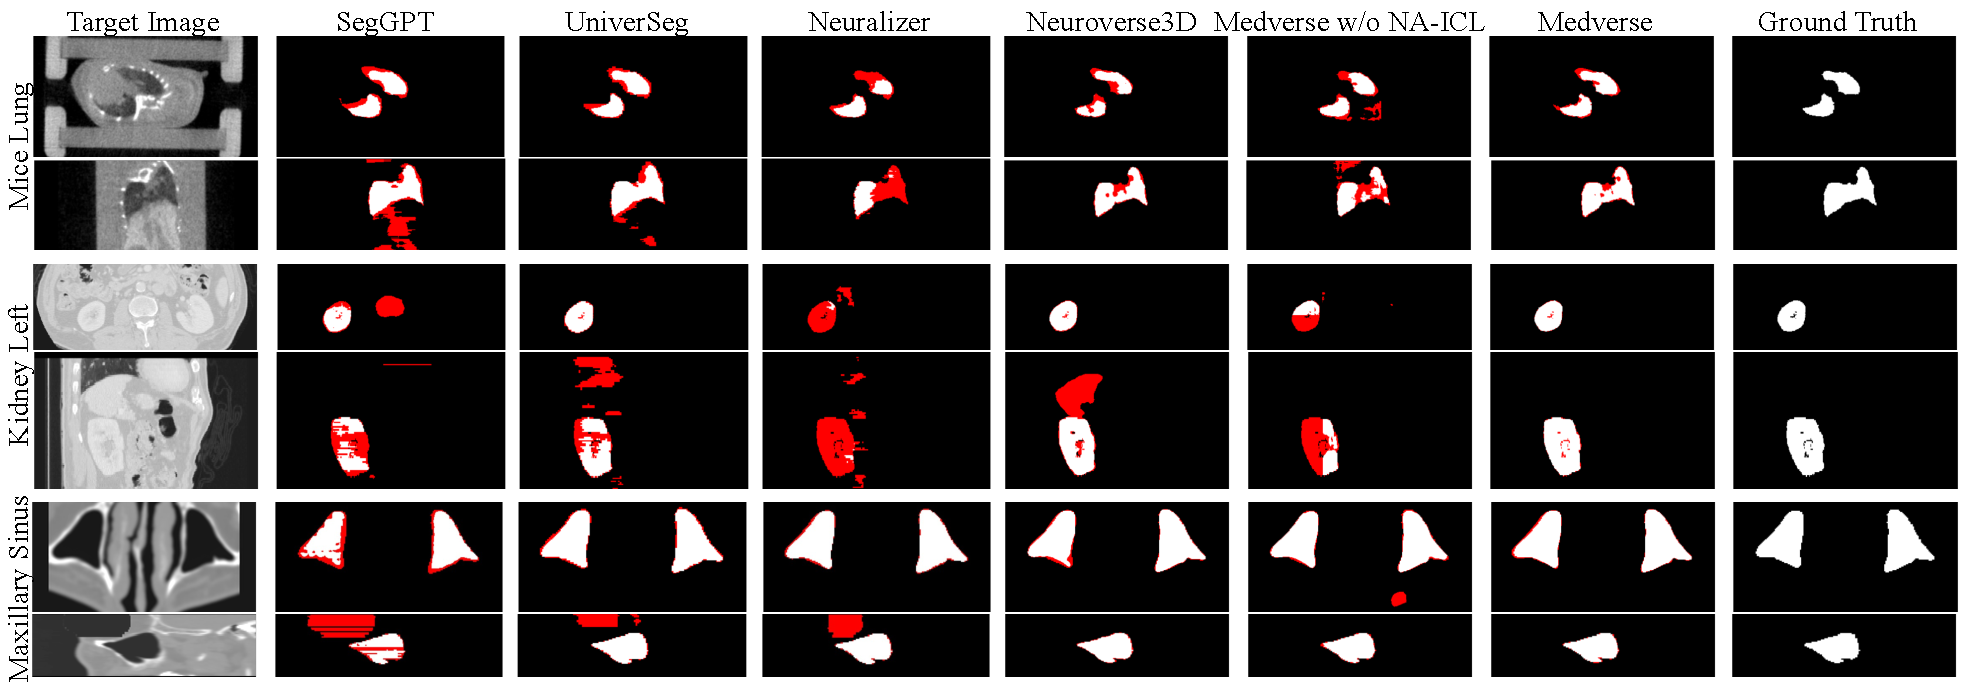
\includegraphics[width=0.95\textwidth]{qualitative1.pdf}
\caption{Qualitative results of ICL models on segmentation tasks. For each 3D segmentation target, results are shown from two views. Red regions indicate segmentation errors. The 2D models take the slice corresponding to the first view as input. Medverse w/o NA-ICL denotes a variant of Medverse without autoregressive processing.}
\label{fig:qualitative1}
\end{figure*}

\subsection{Compared Models}

\noindent\textbf{Medverse.}  
Both the target and context branches are implemented using a five-stage 3D U-Net architecture~\cite{cciccek20163d}.  
Each branch begins with 32 channels in the first stage, with the number of channels doubling at each subsequent stage. The model operates on input patches of size $128 \times 128 \times 128$. In BAM, $p$ is set to 4, and $m$ is set to 66.

\vspace{0.4em}
\noindent\textbf{Task-Specific Models.}  
We compared Medverse against task-specific 3D models.  
Each task-specific model was trained directly on the meta context set of the held-out datasets, thereby mitigating domain shift concerns.  
This setting reflects the conventional practice in clinical environments, where models are trained specifically for a given task.  
Two backbone architectures were evaluated: a 3D U-Net, which shares the same architecture and channel configuration as the Medverse backbone, and the Swin-UNETR~\cite{hatamizadeh2021swin}.  
We assessed performance under both few-shot and fully supervised learning scenarios.

\vspace{0.4em}
\noindent\textbf{Other ICL Models.}  
We compared our method with several state-of-the-art ICL approaches, including Painter~\cite{wang2023images}, SegGPT~\cite{wang2023seggpt}, UniverSeg~\cite{butoi2023universeg}, and Neuralizer~\cite{czolbe2023neuralizer}, all of which are designed for 2D inputs.  
To adapt to 3D, we split each 3D target image into 2D slices and randomly sampled slices from the 3D context set containing the target region to construct the 2D context set.  
The number of context slices was set to 1 for Painter, 8 for SegGPT, 32 for Neuralizer, and 64 for UniverSeg, following the optimal configurations reported in their respective publications.  
The resulting 2D outputs were reassembled into 3D volumes for metric evaluation.  
2D models marked with an asterisk (*) utilize the orthogonal view fusion method from 3 views, which introduces a three-fold increase in computational load.
We also compared with Neuroverse3D~\cite{hu2025building}, an ICL model developed for 3D neuroimaging.  
Due to its limited input resolution of $128 \times 128 \times 128$, we resized the input images to fit Neuroverse3D and rescaled the outputs back to the original resolution for evaluation.  
All models were evaluated using their publicly released pretrained weights.



\begin{figure}[h]
\centering
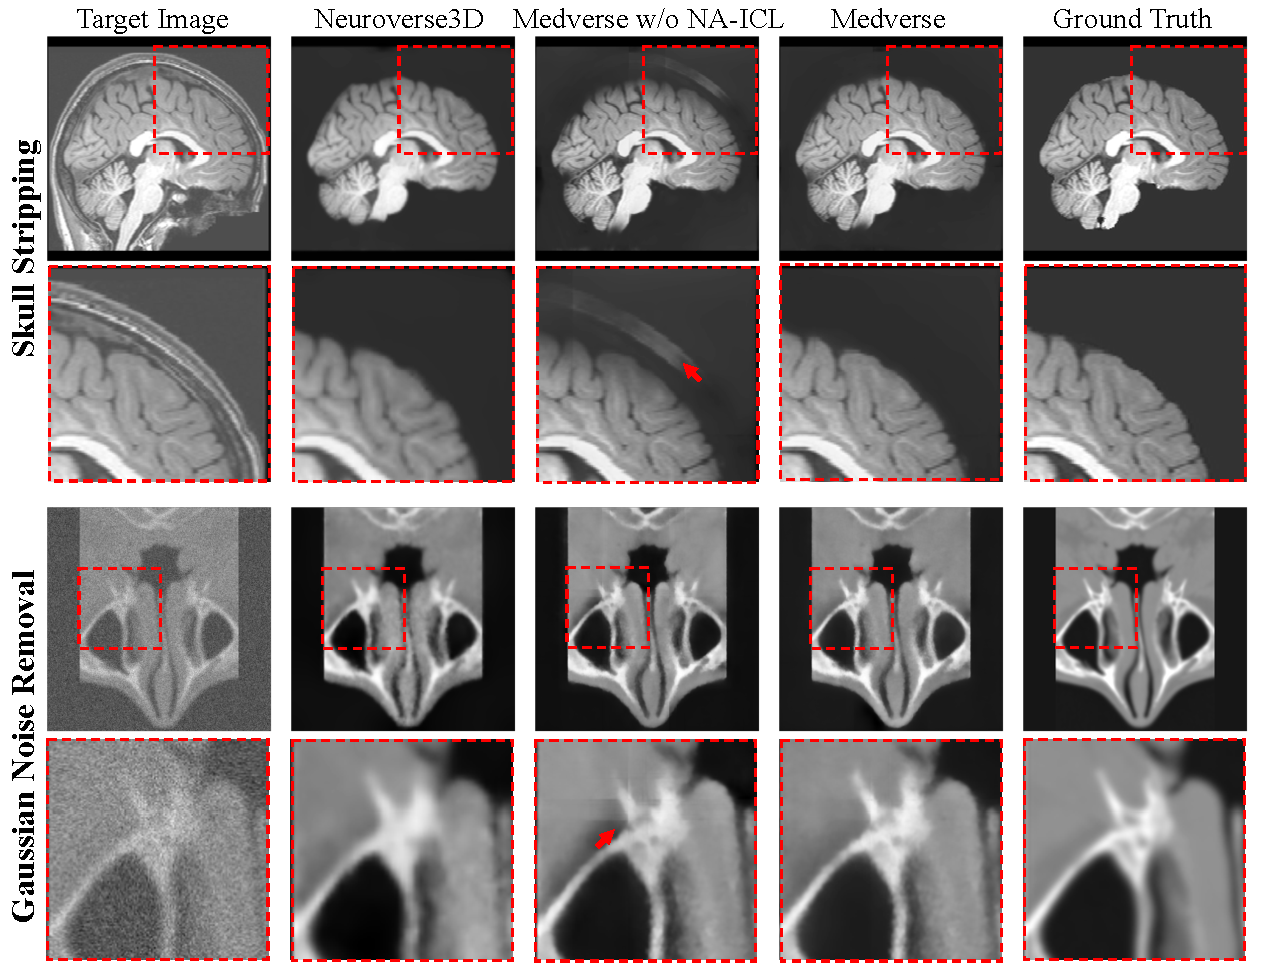
\includegraphics[width=0.45\textwidth]{qualitative2.pdf}
\caption{Qualitative results of 3D ICL models. Medverse w/o NA-ICL denotes the variant of Medverse without autoregressive context. The second row for each task presents zoomed-in views highlighting differences in generated details. Neuroverse3D produces outputs with limited resolution. Red arrows indicate artifacts.}
\label{fig:qualitative2}
\end{figure}

\subsection{Results on Held-Out Dataset}

\vspace{0.4em}
\noindent\textbf{Quantitative Comparison on Segmentation Tasks.}  
Table~\ref{tab:icl_comparison} reports the segmentation performance of the models. Medverse achieves the highest performance among all ICL methods, surpassing the second-best method, Neuroverse3D, by about 6 points in the average Dice score. This improvement can be attributed to Medverse's broader training data coverage and its superior ability to capture fine details enabled by the NA-ICL framework. 2D models, such as UniverSeg and SegGPT, exhibit decreased performance on 3D volumes, primarily due to their tendency to produce false positives in slices that do not contain the target anatomy. When compared to few-shot task-specific models, Medverse achieves similar levels of performance while offering the notable advantage of requiring no task-specific fine-tuning. These results highlight the strong potential and practical value of our method. We further evaluate our model across more classes on the validation set, with results provided in the Supplementary Table 4.

\vspace{0.4em}
\noindent\textbf{Quantitative Comparison on Transformation and Enhancement Tasks.}  
Table~\ref{tab:perturbation_snp} presents the performance of different models on transformation and enhancement tasks. Medverse significantly outperforms other ICL models on tasks such as inpainting and denoising. Although Medverse achieves only a modest improvement of 1.22 PSNR over the second-best Neuroverse3D on average, it preserves the full resolution of the input image, whereas Neuroverse3D limits the resolution of its outputs. Despite being the best among ICL models, Medverse still lags behind the fully supervised 3D U-Net and shows a performance gap compared to the few-shot 3D U-Net.

\vspace{0.4em}
\noindent\textbf{Qualitative Results on Segmentation Tasks.}  
Figure~\ref{fig:qualitative1} presents the segmentation results of different ICL models. The 2D models perform reasonably well on individual slices that contain the target structure but exhibit discontinuities across adjacent slices, and SegGPT and UniverSeg tend to produce false positives in slices without the target. Neuroverse3D alleviates the limitations of 2D processing but struggles to generalize to unseen organ. Medverse w/o NA-ICL refers to applying a sliding window directly, without autoregressive context. In this case, the model lacks access to sufficient global context, leading to unstable predictions. In contrast, Medverse yields the most accurate and fine-grained segmentation results.


\vspace{0.4em}
\noindent\textbf{Qualitative Results on Transformation and Enhancement Tasks.}  
Figure~\ref{fig:qualitative2} illustrates the performance of 3D ICL models on skull stripping and Gaussian noise removal tasks. As shown, Neuroverse3D fails to preserve image resolution, resulting in a loss of fidelity, whereas Medverse effectively retains detailed structures. Without the NA-ICL framework, the model struggles to accurately remove the skull, as having access only to local information increases task difficulty. In the Gaussian noise removal task, stitching artifacts appear as visible lines, which are substantially mitigated when the NA-ICL framework is employed.

Additional qualitative results on segmentation, transformation, and enhancement can be found in the supplementary material.

\vspace{0.4em}
\noindent\textbf{Effect of Context Size.}  
Figure~\ref{fig:context_size} shows how the performance of different ICL models varies with context size. As expected and consistent with prior findings, the performance of all models improves as the context size increases. For Medverse, the Dice score on segmentation tasks improves by 7.28 points with an increasing context size from 1 to 16, while PSNR increases by 0.81 and 1.26 for transformation and enhancement tasks, respectively. The more substantial improvement on segmentation tasks may be attributed to the sparsity of segmentation labels. In contrast, transformation and enhancement tasks typically provide richer semantic guidance per sample, so the marginal benefit from increasing context size is smaller. Furthermore, Medverse consistently outperforms other ICL models across all three kinds of tasks. In transformation tasks, Neuroverse3D performs comparably to Medverse since both skull stripping and modality transformation use neuroimaging data within its training domain. Its slightly lower performance mainly stems from reduced output resolution, unlike Medverse, which preserves full resolution.

\begin{figure}
\centering
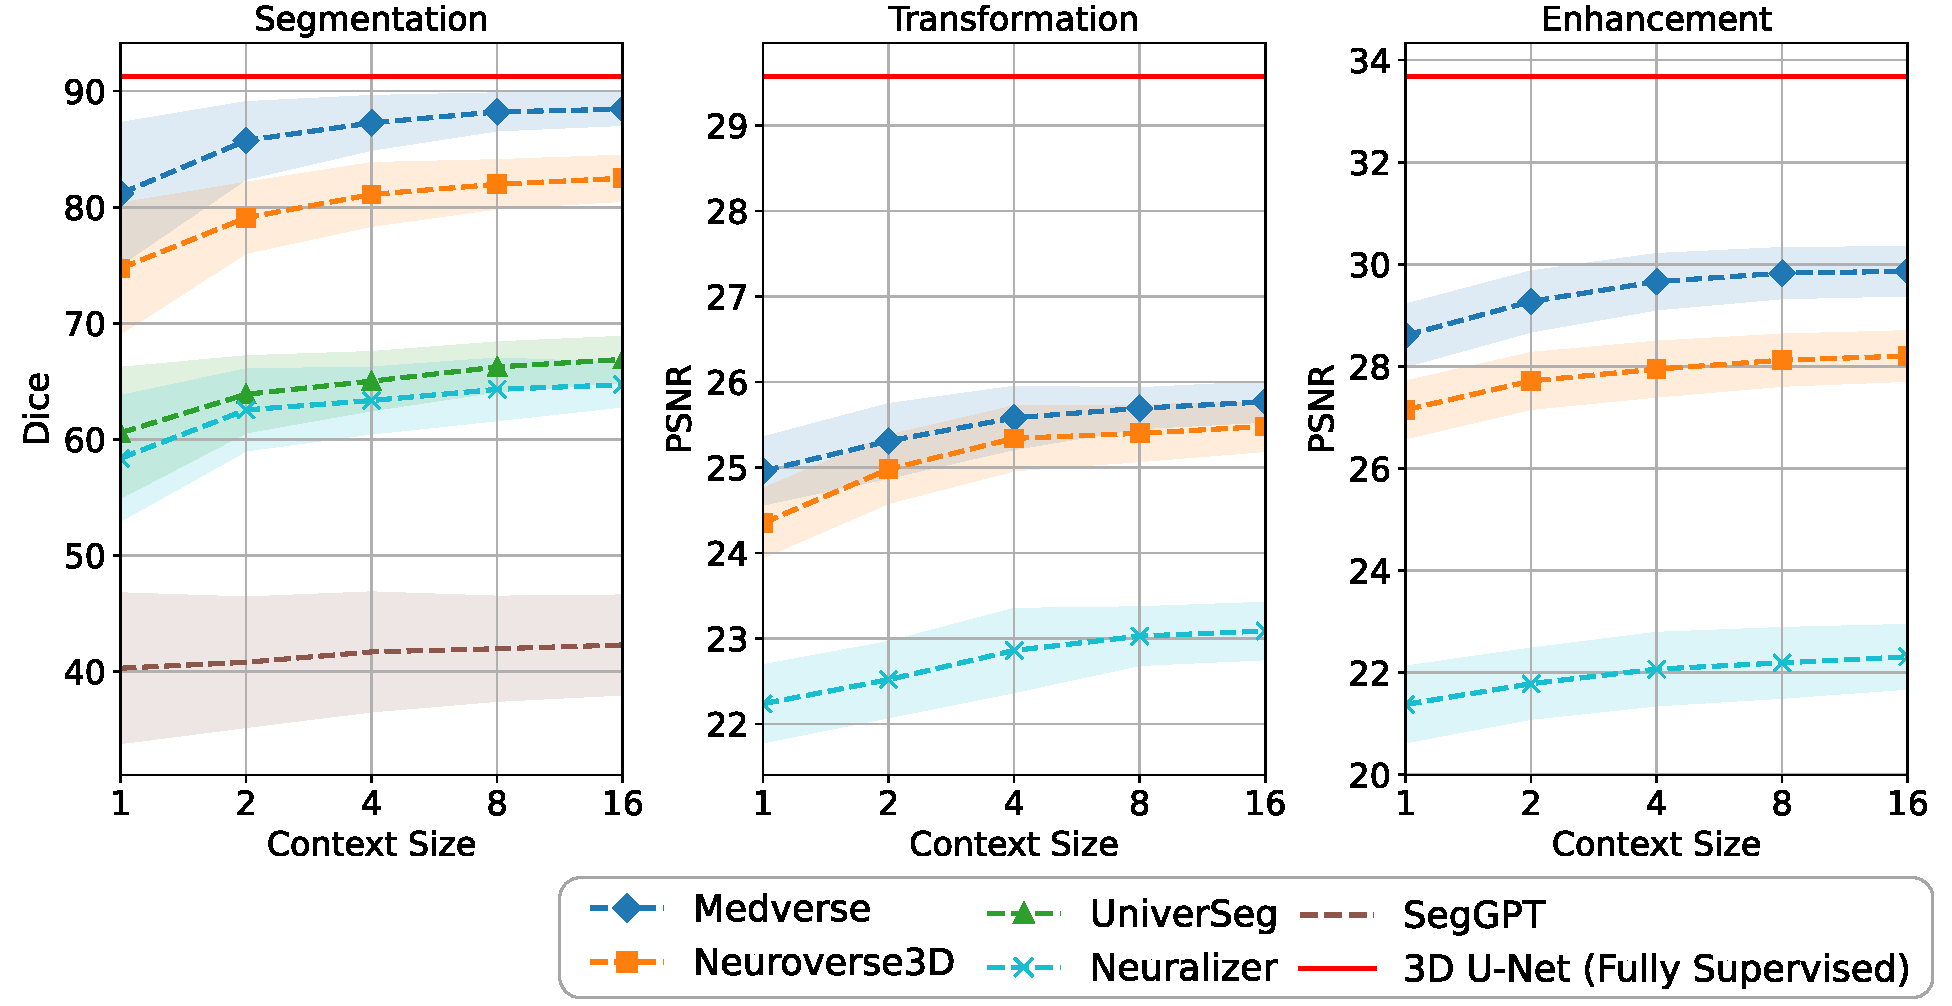
\includegraphics[width=0.473\textwidth]{context_size.pdf}
\caption{Performance comparison of ICL models under varying 3D context sizes.}
\label{fig:context_size}
\end{figure}


\vspace{0.4em}
\noindent\textbf{Computational Efficiency.}  
BAM processes only $4^3$ tokens, adding just $2.01\times10^{-1}$ GFLOPs and $9.18\times10^{-4}$ memory overhead per context pair. In contrast, standard cross-attention with $128^3$ tokens incurs $2.36\times10^6$ GFLOPs and $2.55$ memory overhead, making it computationally impractical. Additionally, our model maintains a fixed inference memory usage of 9.14 GB regardless of context size, enabled by adaptive parallel-sequential context processing. Inference on a $128\times128\times128$ patch with 8 context samples and 1 autoregressive context takes only 1.16 seconds, whereas models like Painter and SegGPT exceed 30 seconds. These properties make our model both efficient and practical for deployment. Full details are provided in the supplemental material.



% \subsection{Ablation Analysis}
\vspace{0.4em}
\noindent\textbf{Ablation Analysis of Key Components.}  
Table~\ref{tab:ablation_bam_autoreg} shows ablations on the BAM module and the NA-ICL framework. Removing NA-ICL, which replaces coarse-to-fine prediction with direct sliding-window inference, leads to a notable drop in segmentation performance. This is due to the limited perspective field of the target image and the loss of global context guidance. For transformation and enhancement tasks, NA-ICL also improves performance, with one contributing factor being its ability to enhance consistency across sliding-window patches. When the BAM module is removed, feature fusion is instead performed via simple concatenation as in~\cite{hu2025building}. The BAM module leads to overall performance improvements due to mitigating the adverse effects caused by spatial misalignment between the context and target images.




\begin{table}[htbp]
\centering
\scriptsize
\setlength{\tabcolsep}{6pt}
\begin{tabular}{cc|ccc}
\toprule
\textbf{BAM} & \textbf{NA-ICL} & \textbf{Seg. (Dice ↑)} & \textbf{Tran. (PSNR ↑)} & \textbf{Enh. (PSNR ↑)} \\
\midrule
             &                & 76.50 & 24.53 & 27.45 \\
\ding{51}    &                & 78.90 & 25.38 & 27.93 \\
\ding{51}    & \ding{51}      & \textbf{87.27} & \textbf{25.58} & \textbf{29.66}   \\
\bottomrule
\end{tabular}
\caption{Ablation study on the BAM module and NA-ICL framework. BAM is replaced with plain feature concatenation when removed, and NA-ICL is replaced with sliding window processing.}
\label{tab:ablation_bam_autoreg}
\end{table}




\section{Conclusion}
In this work, we introduce Medverse, a universal in-context learning model for 3D medical image analysis that performs segmentation, transformation, and enhancement tasks across diverse organs, modalities, and centers. Trained on large-scale heterogeneous data, Medverse generalizes well to unseen domains without task-specific fine-tuning. To enable high-fidelity predictions, we propose the next-scale autoregressive framework for multi-scale anatomical awareness and full-resolution outputs, along with a blockwise Cross-Attention Module for efficient long-range context–target interaction. Extensive evaluations show that Medverse not only outperforms existing ICL models but also establishes a new paradigm for universal 3D medical image processing, effectively addressing the challenge of high-resolution data and revealing the broader potential of ICL in medical imaging.

\noindent\textbf{Limitation.}  Due to limited resources, the current model uses a relatively modest number of parameters and a constrained number of training datasets, leaving room for future scaling to achieve even better performance. Furthermore, conflicts between different tasks may not have been fully resolved. For instance, exclusively utilizing the segmentation Dice loss while discarding the transformation and enhancement tasks could potentially yield superior segmentation results. Therefore, how to more effectively unify the transformation and enhancement tasks with the segmentation task warrants further investigation.


% This work takes a step toward building practical, generalizable, and task-flexible AI systems for medical image understanding.




